% =====================================================================
% Part 4 - Second foundation model (ChemBERTa-2)
% Daniel Morales & Miguel Quijada
%
% Standalone two-column document. To merge into the group report,
% delete the preamble and everything outside \section{...}, and
% \input{} this file from main.tex.
%
% Needs: booktabs, graphicx
% =====================================================================
\documentclass[10pt,twocolumn,a4paper]{article}
\usepackage[utf8]{inputenc}
\usepackage[T1]{fontenc}
\usepackage[margin=2cm]{geometry}
\usepackage{booktabs}
\usepackage{graphicx}
\usepackage{amsmath}
\setlength{\columnsep}{0.7cm}
\pagestyle{empty}

\begin{document}

\section{Second foundation model: ChemBERTa-2}

\subsection{Model and integration}

ChemBERTa-2 is a RoBERTa encoder pretrained on SMILES strings. It
contrasts cleanly with Atom-JEPA: it reads the molecule as 1D text
rather than 3D geometry, so it needs no conformers, and it is small
(3.3M parameters, 384-dimensional embeddings). We use the
\texttt{DeepChem/ChemBERTa-77M} checkpoints.

Two checkpoints exist, pretrained on different objectives. \textbf{MLM}
masks tokens of the SMILES string and predicts them from context, so it
learns the grammar of valid molecules. \textbf{MTR} instead predicts 200
computed physicochemical descriptors, so it learns to map structure to
properties. Their load reports confirm this: MLM ships
\texttt{lm\_head} layers, MTR ships \texttt{regression.*} layers with
normalisation statistics.

Integration follows the starter code's model interface, with
tokenisation in the collate function. Because the encoder emits one
vector \emph{per token}, a pooling step reduces them to one vector per
molecule, either the \texttt{CLS} token or the mask-weighted
\texttt{mean}, before the MLP readout.

\subsection{Methodology}

The validation metric fluctuates markedly between epochs while the
training loss falls smoothly (Fig.~\ref{fig:curves}). Since the loop
keeps the best epoch by validation, it selects the minimum of a noisy
series, which biases the reported score downwards, so a single run is
not a reliable measurement. We therefore ran every configuration behind
a decision with three seeds and report mean $\pm$ standard deviation.
The spread is roughly $\pm 0.01$, so we treat differences below $0.02$
ST-RAE as noise. All decisions use validation only; test was evaluated
once, at the end.

\subsection{Adapting the MLM checkpoint}

The starter configuration inherits \texttt{encoder\_lr}~$=10^{-5}$ from
Atom-JEPA. For ChemBERTa this is an order of magnitude too low: sweeping
$10^{-5}$ to $5\times10^{-4}$ gives a U-shaped curve with a minimum at
$10^{-4}$ and a total range of $0.076$, improving validation ST-RAE from
$0.900 \pm 0.013$ to $0.829 \pm 0.018$.

Learning rate and epoch budget interact: the best epoch is 13 at
$10^{-5}$, 4 from $2\times10^{-5}$ upwards and 2 at $5\times10^{-4}$.
Training for 60 epochs instead of 20 reproduces the result exactly.
Freezing the encoder costs $0.118$ ST-RAE ($0.809 \rightarrow 0.927$),
so the MLM representation clearly needs to adapt.

Pooling matters as well: \texttt{mean} beats \texttt{CLS}
($0.792 \pm 0.008$ vs $0.829 \pm 0.018$) and is more stable across
seeds. This is expected for an MLM-pretrained encoder, where the
\texttt{CLS} token receives no pressure to summarise the sequence; the
pooler weights are in fact absent from the checkpoint.

\subsection{Effect of the pretraining objective}

Repeating the checkpoint $\times$ pooling grid at
\texttt{encoder\_lr}~$=10^{-4}$ (Table~\ref{tab:grid}) shows that MTR
outperforms MLM on both tasks, and that the pooling effect
\emph{reverses}: \texttt{mean} is better under MLM, \texttt{CLS} under
MTR. This follows from the objectives. MTR's regression head predicted
all 200 descriptors from the sequence summary, so its \texttt{CLS}
token is trained to be informative, whereas MLM's is not.

\begin{table}[t]
  \centering
  \caption{Validation performance of the checkpoint $\times$ pooling
  grid at \texttt{encoder\_lr}~$=10^{-4}$, single seed.}
  \label{tab:grid}
  \begin{tabular}{llcc}
    \toprule
    Checkpoint & Pooling & ST-RAE $\downarrow$ & MCC $\uparrow$ \\
    \midrule
    MLM & CLS  & 0.809 & 0.188 \\
    MLM & mean & 0.794 & 0.251 \\
    MTR & CLS  & \textbf{0.734} & \textbf{0.299} \\
    MTR & mean & 0.746 & 0.241 \\
    \bottomrule
  \end{tabular}
\end{table}

An ablation isolates the contribution of pretraining itself: the same
architecture with randomly initialised weights reaches $0.982$ on
regression, which is what predicting the training mean achieves
($0.983$), and MCC $0.000$ on classification, i.e.\ predicting the
negative class everywhere. All of the performance comes from
pretraining, none from the architecture.

\subsection{MTR is robust to how it is adapted}

Repeating the learning-rate sweep on MTR gives a range of only $0.019$
across two orders of magnitude, against $0.076$ for MLM: within our
noise threshold, so no setting is significantly better than another.
Freezing the encoder costs $0.026$ on regression and $0.013$ MCC on
classification, against $0.118$ for MLM. An aggregate analysis across
all 64 runs agrees, finding neither effect significant
($p = 0.40$ and $p = 0.21$).

Three independent observations therefore point the same way.
\textbf{MLM encodes structure and needs substantial adaptation; MTR
already encodes properties and needs very little.} We kept
$10^{-4}$ for continuity with the earlier experiments, not because it
is optimal: under MTR the choice does not matter.

\subsection{Final configuration and results}

The selected configuration is the MTR checkpoint with \texttt{CLS}
pooling, \texttt{encoder\_lr}~$=10^{-4}$ and a fine-tuned encoder
(Table~\ref{tab:final}). It is also the most stable across seeds
($\pm 0.005$).

\begin{table}[t]
  \centering
  \caption{Progression of validation scores and test results of the
  selected configuration. Regression is macro ST-RAE (lower is better),
  classification is mean MCC (higher is better).}
  \label{tab:final}
  \begin{tabular}{lcc}
    \toprule
    Configuration & Regression & Classif. \\
    \midrule
    \multicolumn{3}{l}{\emph{Validation}} \\
    MLM + CLS, $10^{-5}$  & $0.900 \pm 0.013$ & 0.142 \\
    MLM + mean, $10^{-4}$ & $0.792 \pm 0.008$ & 0.251 \\
    MTR + CLS, $10^{-4}$  & $\mathbf{0.730 \pm 0.005}$ & \textbf{0.299} \\
    \midrule
    \multicolumn{3}{l}{\emph{Test}} \\
    MLM + mean, $10^{-4}$ & 0.810 & 0.193 \\
    MTR + CLS, $10^{-4}$  & \textbf{0.798} & \textbf{0.232} \\
    \bottomrule
  \end{tabular}
\end{table}

\begin{figure}[t]
  \centering
  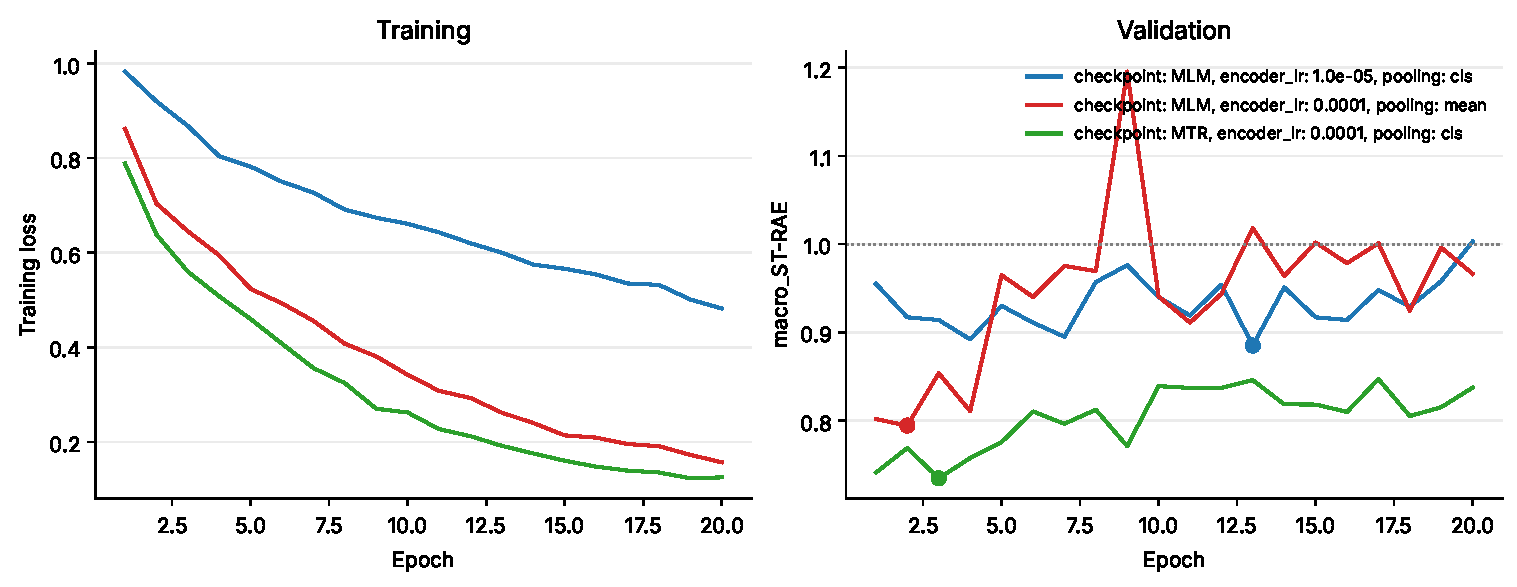
\includegraphics[width=\columnwidth]{chemberta_curves.pdf}
  \caption{Training loss and validation ST-RAE per epoch for the
  starting configuration, the tuned MLM model and the final MTR model.
  All three overfit within a few epochs; the validation curve
  fluctuates throughout, which motivates the multi-seed protocol.}
  \label{fig:curves}
\end{figure}

MTR's advantage shrinks on test: $0.064$ on validation against $0.012$
on test for regression. It remains the better model on both tasks, so
the selection was correct, but part of the validation margin was
specific to the split used to choose it, which is the expected cost of
selecting among many configurations. The classification advantage holds
up better ($0.232$ vs $0.193$).

\subsection{Limitations}

The aggregate hides a split outcome. CYP3A4 is consistent between
validation and test (AUROC $0.762$ vs $0.771$), whereas CYP2D6
collapses (MCC $0.211 \rightarrow 0.036$, AUROC $0.530$) with only
around 60 positive cases; its regression $R^2$ of $0.05$ tells the same
story, so the apparent validation score was noise. Classification is
further limited by imbalance: with roughly 20\% positives the model
rarely exceeds the fixed $0.5$ threshold, ranking well but deciding
poorly, and no alternative threshold rule improved on it.

\end{document}
